\documentclass{lkx_thesis}
\usepackage{lkx_thesis}
\usepackage{lkx_diagrams}

\title{Exotic Spheres}
\subtitle{Some subtitle}
\author{Lev Kruglyak}

\department{The Department of Mathematics}
\degree{Bachelor of Arts with Honors}
\subject{Mathematics}

\university{Harvard University}
\location{Cambridge, Massachusetts}
\date{April 2025}

\titlegraphic{graphics/title/hopf4.png}

\advisor{Dr. Stephen McKean}
\advisor{Professor Michael Hopkins}

\begin{document}

\makeatletter
{
	\begin{titlepage}
		\begin{center}
			\hfill
			\vfill
			{\Huge\scshape{\@title}}\\[2ex]
			{\Large\@subtitle}\\[0.5in]

			\includegraphics[width=3in]{\@titlegraphic}\\[0.5in]

			{\scshape

			{by\\[1em]}
			{\large\scshape{\@author}}\\[1em]
			{advised by\\[1em]}
			{\large\scshape\advisorlist}\\[0.5in]

			{A thesis presented to \\[1em]}
			% {\bfseries\large\textsl{\@university}\\[1em]}
			{\large\scshape{\@university}\\[1em]}
			in partial fulfillment of the\\
			requirements for the degree of\\[1em]

			{
			\large
			% {\bfseries\textsl\@degree}\\
			{\scshape\@degree}\\
			in the subject of
			% {\bfseries\textsl\@subject}\\[1em]
			{\scshape\@subject}\\[1em]
			}
			%
			% {\@location}\\
			% {\@date}\\
			}
			\vfill
		\end{center}
	\end{titlepage}
}
\makeatother
\pagebreak


\lkxtoc

% Epigraph
\begin{flushleft}
	\textsl{Existence plays a mischievous game with us,}\\
	\textsl{as though to tease and provoke us. In the }\\
	\textsl{midst of knowledge there yet again arises }\\
	\textsl{the mystery; in the midst of contemplation}\\
	\textsl{the riddle gains new strength.}\\
	\rule[0pt]{19.5em}{0.5pt}\\
	-- \textsc{Joseph Soloveitchik}\\
	% \phantom{-- }\textsl{``Ish ha'Halakhah''}
	\vspace{2em}
\end{flushleft}

% \begin{flushleft}
% 	\textsl{One might say that, in whatever manner God might have}\\
% 	\textsl{created the world, it would always have been in accordance}\\
% 	\textsl{with a certain general order. But God has chosen the most}\\
% 	\textsl{perfect world, that is, the one which is at the same time}\\
% 	\textsl{the simplest in hypothesis and richest in phenomena.}\\
% 	\rule[0pt]{26em}{0.5pt}\\
% 	-- \textsc{Gottfried Leibniz}\\
% 	% \phantom{-- }\textsl{``Discours de m\'etaphysique''}
% 	\vspace{2em}
% \end{flushleft}

Before talking about exotic spheres, I want to talk about symmetry.

% Projective plane analogy with torsion (Z/2 vs Z/28)

% Humanity has been fascinated by questions of physical space for thousands of years. As with many areas of math, this burning curiosity first arose in antiquity out of practical concerns: measuring the volume of a cylindrical grain silo, computing the circumference of the earth, predicting the motion of celestial bodies, etc. In order to make these questions precise in the idealized world of mathematical forms, we must first make our intuitive notions of space precise. 
% Euclidean geometry, for instance, takes place on an infinite continuum of points, and comes with a way to measure distances and angles. It also contains a strong notion of parallelism -- starting at a point and choosing a direction gives a straight line which extends indefinitely. If we pick any other point not this line, travelling in that same direction gives us a parallel, non-overlapping line.
%
% To us, physical space at the scales which we inhabit is so intuitively Euclidean, and so baked into the very structures of our mind that it's difficult to imagine where our assumptions might be biased. We tend to think of space as infinite and flat, just as Euclid's axioms describe. At the scale of daily life this is an accurate model, but at the scale of the Earth it completely falls apart. The Earth is neither infinite nor flat, and \emph{any} straight line path will eventually bring you back to your starting point. 
% And that's only the two-dimensional surface of the spherical Earth. What if the universe itself was finite, curving in on itself rather than extending indefinitely? You might imagine zooming into the depths of the cosmos with a super-powered telescope only to see familiar galaxies, and eventually Earth itself peering back at you.
% Even worse, what if space was non-orientable? Not only could flying in a straight path bring you right back to where you started, but you would find that upon your arrival the very notions of right and left seem to have swapped places -- as though you've entered a mirror world. All languages become illegible to you since they are now backwards from your perspective, a birthmark which used to be on the left side of your face appears to everyone else to be on your right. Only another trip along the same course you originally took is able to flip everything back.
%
% \begin{figure}
% 	\centering
% 	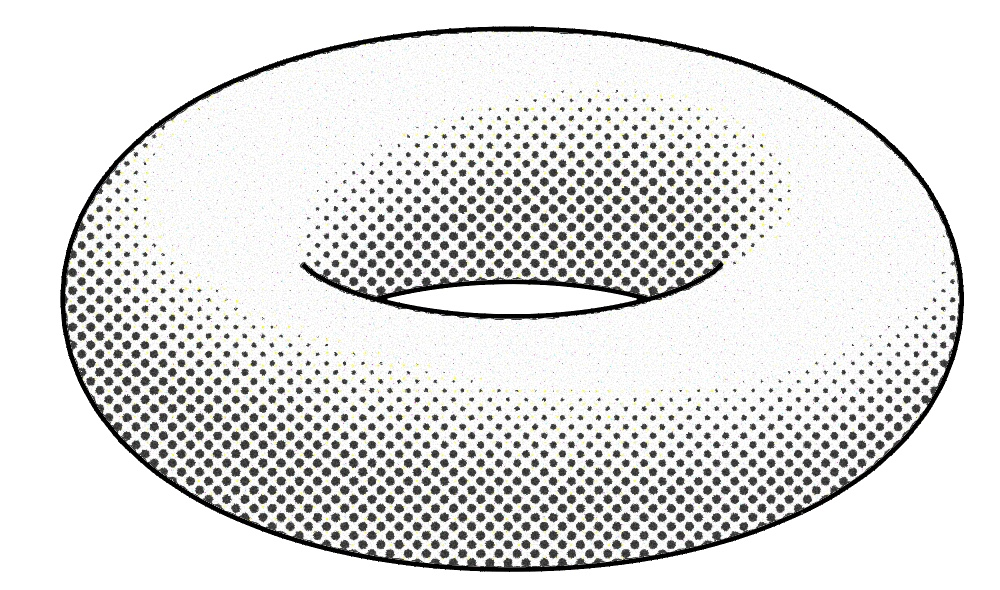
\includegraphics[scale=0.3]{graphics/diagrams/torus_non_vanishing_vector_field/result.jpg}
% 	\vspace{1em}
% 	\caption{A torus.}
% \end{figure}
%
% By relaxing our assumptions about the shape of space, geometry begins to quickly fill up with many such counter-intuitive non-Euclidean spaces and they find applications in unexpected places. Take for instance 
%
% \hspace{1em}
% % Many such axiomatic foundations exist, and lead 
%
% Let's start with the simple case of Euclidean space (think of a plane for instance) by describing some of its essential aspects. First and foremost Euclidean space is comprised of infinitely many points which \emph{extend continuously}, which informally means that Euclidean space is equipped with a qualitative concept of ``closeness''. Among other things, this 
%
% Euclidean space also comes with the stronger, quantitative notion of closeness -- this is known as \defn{distance}. A distance metric assigns to each pair of points a non-negative real number.

% \pagebreak

% \todo{The geometries they worked in were mostly flat, i.e. Euclidean and they relied on entirely (analytical?) methods to derive spatial relationships}
%
% \todo{Take a step back and see what data we have.}
%
% Classical geometry works in affine space, so we have: continuity of space, distance,  translation and homotethy. Translation gives us a global parallelism.
%
% Introduction of curvature
%
% Intrinstic  geometry via Theorema Egregium
%
% Symplectic manifolds, spin manifolds -> corresponding to physics
%
% Ehrlangen program

% At the scales they worked at, reality was best modelled by a plane or a (flat) three dimensional space.

% Homotopy classes of spaces
%
% PL manifolds
%
% During my last summer before graduating college, I went with some friends on a mountaineering trip up Banner peak, a picturesque mountain in the eastern Sierra Nevada range of California. 
% %
% % As we descended the glacier towards our base camp, ice axes in hand, I 
% So how \emph{do} we study objects which we can't touch, see, or possibly hope to visualize in their full complexity?
%
% There are two levels to understanding.
% \begin{enumerate}
% 	\item First, we
% \end{enumerate}
%
% Understanding an object by how it behaves with respect to other objects.
% \todo{spectral lines of atoms}
%
% One of the earliest methods to ``fingerprint'' topological objects was discovered by Euler.

% \cite{hatcher2002}

% \begin{flushleft}
% 	\textsl{There is geometry in the humming of the strings,}\\
% 	\textsl{and there is music in the spacing of the spheres.}\\
% 	\rule[0pt]{21em}{0.5pt}\\
% 	-- \textsc{Pythagoras}\\
% 	\vspace{2em}
% \end{flushleft}

\begin{flushleft}
	\textsl{God created the integers,}\\
	\textsl{the rest is the work of man.}\\
	\rule[0pt]{13em}{0.5pt}\\
	-- \textsc{Leopold Kronecker}\\
	\vspace{2em}
\end{flushleft}

\todo{introduce, motivate, provide historical context.}

\begin{conjecture}[Poincar\'e Conjecture]
	Every closed topological $3$-manifold which is simply connected is homeomorphic to the $3$-sphere $S^3$.
\end{conjecture}

\begin{definition}
	If $U\subset \R^n$ is an open subset, a function $f : U \to \R^m$ is said to be \defn{smooth}[smooth function] if all partial derivatives of $f$ exist to all orders.
\end{definition}

\begin{definition}
	A \defn{smooth structure} $\mathscr{S}$ on a topological manifold $M$ (possibly with boundary) is a collection of charts $\mathscr{S}=\{(U_\alpha, \varphi_\alpha)\}_{\alpha\in I}$ such that the transition functions
	\begin{equation}\label{eq:transition-function}
		\lkxfunc{\varphi_\alpha\varphi_\beta^{-1}}{\varphi(U_\alpha\cap U_\beta)}{\R^n\textrm{ or } \R^{n-1}\times [0,\infty)}
	\end{equation}
	are smooth for all $\alpha,\beta\in I$. We require that $\mathscr{S}$ be maximal with respect to this property, i.e. the addition of any chart $(U,\varphi)$ not in $\mathscr{S}$ breaks the smoothness of \cref{eq:transition-function}.
\end{definition}
% A smooth structure gives rise to tangent spaces -- at each point of the3manifold there is a notion of infinitesimal direction, and the set of all such infinitesimal directions forms a vector space of tangent vectors. \todo{physics}

While the class of smooth manifolds offers a tempting for context for the exploration of the shape of space, it is far from the only type of manifold one can define. Another equally valid category in which to study topology of manifolds is $\Pl$, or the piecewise linear category. A $\Pl$ structure on a manifold consists of

\begin{conjecture}[Generalized Poincar\'e Conjecture]
	Letting $\mathscr{C}$ be either $\Top$, $\Pl$, or $\Diff$, any $\mathscr{C}$-manifold which is homotopy equivalent to the $n$-sphere $S^n$ is also $\mathscr{C}$-isomorphic to $S^n$.
\end{conjecture}

\begin{conjecture}[Hauptvermutung]
	\todo{this}
\end{conjecture}

\todo{questions about equivalence of TOP, PL, and DIFF}

\todo{goal of this chapter is provide some fundamental concepts needed to begin working on the problem}

\subsection{Morse Theory}

While a fully comprehensive introduction to Morse theory is outside of the scope of this thesis, we'll include a basic overview for completeness. A great classical introduction to Morse theory can be found in Milnor's book on the subject \cite{milnor1963morse}.

If $f : M \to \R$ is a smooth function on a manifold $M$, the points $p\in M$ where the differential $df_p : \T_p M \to \T_{f(p)} \R = \R$ vanish are known as \defn{critical points}, and their images in $\R$ are called \defn{critical values}. In terms of local coordinates $\{x^1,\ldots, x^n\}$ at $p$, this means that
\[
	\frac{\partial f}{\partial x^1}=\cdots=\frac{\partial f}{\partial x^n} = 0.
\]
A critical point $p\in M$ is said to be \defn{non-degenerate}[non-degenerate point] if the matrix
\[
	\everymath={\displaystyle}
	\renewcommand*{\arraystretch}{2}
	H_f(p) = \begin{pmatrix}
		\frac{\partial^2 f}{\partial x^1\partial x^1} & \cdots &
		\frac{\partial^2 f}{\partial x^1\partial x^n}                   \\
		\vdots                                        & \ddots & \vdots \\
		\frac{\partial^2 f}{\partial x^n\partial x^1} & \cdots &
		\frac{\partial^2 f}{\partial x^n\partial x^n}                   \\
	\end{pmatrix}(p)
\]
is invertible at $p$. This is called the \defn{Hessian matrix} of $f$ at $p$, and in this formulation depends on our chosen coordinate system.
There is a coordinate independent way to define the Hessian as a symmetric bilinear form on $\T_p M$ which makes the coordinate invariance of the condition of non-degeneracy manifestly apparent.

\begin{definition}
	The \defn{index}[index of a function] of $f$ at a point $p$ is the maximal dimension of a subspace on which $H_f(p)$ is negative definite, i.e. it is the dimension of $\{v\in \R^n \mid v^\intercal H_f(p) v < 0\}.$
\end{definition}

The index of a function at a point essentially describes the ``shape'' of the function out of a list of finitely many possible shapes. Remember, the index of a function on an $n$-dimensional manifold must be an integer between $0$ and $n$. For instance, in the case of a surface there are three possible shapes -- when both coordinates curve up we get a bowl facing up, when one curves up and one curves down we get a saddle, and when both coordinates curve down we get a bowl facing down. These shapes correspond to indices of $0$, $1$, and $2$ respectively.
\begin{figure}[ht]
	\centering
	\todo{draw figure}
	\medskip
	\caption{An upward bowl, saddle, and downward bowl.}
\end{figure}

The fundamental lemma of Morse theory makes rigorous this notion of a manifold having a shape dictated by a real-valued function -- there is always a local coordinate system which puts the function into a standard form depending on the index.

\begin{lemma}[Morse Lemma]\label{lemma:morse}
	Let $p$ be a non-degenerate critical point of $f$. There is a local coordinate system $(y^1,\ldots, y^n)$ at $p$ such that
	\[
		f(y^1,\ldots, y^n)=f(0)-\left[(y^1)^2 + \cdots + (y^{\ell})^2\right] + \left[(y^{\ell + 1})^2 + \cdots + (y^n)^2\right].
	\]
	where $\ell$ is the index of $f$ at $p$.
\end{lemma}
\begin{proof}
	Let's assume without loss of generality that $f(p)=0$. Given any local coordinate system $(x^1,\ldots, x^n)$ at $p$, we can write
	\[
		f(x^1,\ldots, x^n) = \sum_{1\leq j \leq n} x^j g_j(x^1,\ldots, x^n)
	\]
	where $g_j$ are functions satisfying $g_j(0)=(\partial f / \partial x^j)(0)$. 
	This can be achieved by setting $g_j(x_1,\ldots, x_n) = \int_0^1 (\partial f/\partial x^j)(tx_1, \ldots, tx_n)\,dt$. Since $p$ is a critical point

	\todo{basic idea}
\end{proof}

Inspired by this lemma, we might call a function $f : M \to \R$ a \defn{Morse function} if all critical points are non-degenerate.

\begin{corollary}
	Non-degenerate critical points are isolated.
\end{corollary}

For a brief demonstration of the power of the Morse lemma, we'll prove Reeb's theorem, a Morse theoretic criterion for a compact manifold to be homeomorphic to a sphere. Throughout the thesis, we'll usually defer to the more powerful $h$-cobordism theorem to prove that a manifold is homoemorphic to a sphere. However, it is useful to not always rush for the flamethrower when trying to kill a fly -- a simple swatter might do the trick. We'll see a direct application of this lighter theorem in \cref{sec:first-exotic-sphere}.

\begin{theorem}[Reeb]\label{thm:reeb}
	If $M$ is a compact manifold and $f$ is a Morse function with exactly $2$ critical points, then $M$ is homeomorphic to a sphere.
\end{theorem}
\begin{proof}
	Firstly, by compactness of $M$ we can find a global minimum $f(x_0)$ and global maximum $f(x_1)$ for some distinct points $x_0$ and $x_1$ (otherwise the function would be constant and not a Morse function with $2$ critical points). We can normalize the function $f$ to have $f(x_0)=0$ and $f(x_1)=1$ without loss of generality. It follows that $x_0$ is a non-degenerate critical point of index 0 and $x_1$ is a non-degenerate critical point of index $n$.
	By the Morse lemma (\ref{lemma:morse}), there is a neighborhood $x_0\in U_0$ with local coordinates $\{y^1,\ldots, y^n\}$ such that 
	\[
			f(y^1,\ldots, y^n) = (y^1)^2 + \cdots + (y^n)^2.
	\]
	This gives a Riemannian metric $(dy^1)^2+\cdots+(dy^n)^2$ on $U$ which can be extended to all of $M$ by partitions of unity.
	% A Riemannian metric on a manifold $M$ determines an isomorphism $\T^\d M \cong \T M$, and hence an isomorphism $\Omega^1(M)=\Gamma(\T^\d M) \cong \Gamma(\T M)=\X(M)$ between the space of $1$-forms and the space of vector fields. Composing this isomorphism with the exterior derivative $d : \Omega^0(M)\to \Omega^1(M)$ gives the gradient operator $\nabla : \Omega^0(M) \to \X(M)$ sending a function to its vector field. 

	Given a Riemmanian structure, there is a gradient operator $\nabla : \Omega^0 \to \X(M)$ sending functions to vector fields.
	In our case, the vector field $\nabla f$ is non-zero everywhere except for at $x_0$ and $x_1$. We thus have a normalized vector field $\nabla f/\|\nabla f\|^2$
	defined everywhere except for at $x_0$ and $x_1$. Let $\varphi_t : M \to M$ be the global flow corresponding to this vector field, i.e. the unique solution to the differential equation
	\[
	\left.\frac{d\varphi_t(p)}{dt}\right|_{t=0} = \frac{\nabla f(p)}{\|\nabla f(p)\|^2}
	\]
	for all $p\in M\setminus \{x_0,x_1\}$. By the chain rule, it follows that
	\[
		\frac{d(f\circ \varphi_t(p))}{dt}=\left\langle \frac{d\varphi_t(p)}{dt}, \nabla f\right\rangle = \left\langle \frac{\nabla f}{\|\nabla f\|^2}, \nabla f\right\rangle=1.
	\]
	In particular, this implies that $f\circ \varphi_t(p) = f(p)+t$. 

	\todo{finish the proof}
\end{proof}

The basic ideas used in the proof of Reeb's theorem can be radically generalized.

\begin{definition}
	For any $a\in \R$, the \defn{level set} of a smooth function $f : M \to \R$ is the set 
	\[
		M_a = f^{-1}(-\infty, a] = \{ p\in M \mid f(p)\leq a)\}.
	\]
\end{definition}

\begin{figure}
\end{figure}

\begin{theorem}
	Let $f : M \to \R$ be a smooth function and suppose $f^{-1}[a,b]$ contains no critical points of $f$ for real numbers $a<b$. Then $M_a$ is diffeomorphic to $M_b$. Furthermore $M_a$ is a deformation retract of $M_b$.
\end{theorem}

\begin{theorem}
	Let $f : M \to \R$ be a smooth function and let $p$ be a non-degenerate critical point of index $\ell$. Letting $c=f(p)$, suppose that $f^{-1}[c-\epsilon, c+\epsilon]$ is compact and contains no critical points of $f$ aside from $p$. For sufficiently small $\epsilon$, the level set $M^{c+\epsilon}$ has the homotopy type of $M^{c-\epsilon}$ with an $\ell$-cell attached.
\end{theorem}

\begin{theorem}
	If $f$ is a Morse function with compact level sets (for instance if $M$ is compact), then $M$ has the homotopy type of a CW-complex with a cell in each dimension $\ell$ for each critical point of index $\ell$.
\end{theorem}

\todo{finish}

\subsection{Cobordism}\label{sec:cobordism}

The basic principle of cobordism is to declare two manifolds equivalent if there is a manifold a dimension higher which connects the two manifolds. As an equivalence relation, cobordism is generally far looser than the notions of homoemorphism or diffeomorphism. In most dimensions, classifying manifolds up to strict notions of homeomorphism or diffeomorphism is provably impossible -- from a computational complexity standpoint such problems are undecidable. Cobordism on the other hand is loose enough to allow for a full classification.

\begin{remark}
	Note that the implied compactness assumption throughout the thesis is important here, otherwise any manifold $M$ is trivially the boundary of $M\times [0,\infty)$. 
\end{remark}

\begin{definition}
	An \defn{unoriented cobordism} between closed $n$-manifolds $M_1$ and $M_2$ is an $(n+1)$-manifold $W$ with $\partial W = M_1\sqcup M_2$. We use the notation $W : M_1\bord M_2$ to refer to the cobordism.
\end{definition}

\begin{definition}
	An \defn{oriented cobordism} between closed oriented $n$-manifolds $M_1$ and $M_2$ is an oriented $(n+1)$-manifold $W$ with $\partial W = M_1\sqcup (-M_2)$. We use the notation $W : M_1\sobord M_2$ to refer to the cobordism.
\end{definition}

\begin{example}
	Within some category of 
\end{example}

\begin{figure}[ht]
	\centering
	\import{graphics/temp-diagrams/}{pair-of-pants.pdf_tex}
	\caption{A cobordism $W$ between $S^1$ and $(S^1\sqcup S^1)$.}\label{fig:pair-of-pants}
\end{figure}

For a simple example of a cobordism between a circle and a disjoint union of circles, see \cref{fig:pair-of-pants}. Note that this cobordism could be made much simpler by removing the handle. Simplifying cobordisms in this way is one of the major applications

\begin{definition}
	The \defn{$\bm{k}$-th oriented cobordism group}[oriented cobordism group] $\Omega^\SO_k$ is the abelian group of oriented cobordism classes of closed $k$-manifolds\footnote{We do not require manifolds to be connected in this definition.}
	under disjoint union. The identity component is the empty set $\varnothing$, and negation is given by reversing orientation. Similarly, the \defn{$k$-th unoriented cobordism group}[unoriented cobordism group] $\Omega_k$ is the abelian group of cobordism classes of closed $k$-manifolds under disjoint union.
\end{definition}

Note that the oriented cobordism group can be thought of as a $\Z$-module, with multiplication action on a closed manifold $M$ given by
\[
	n \cdot M = \begin{cases} M\sqcup \cdots \sqcup M & n > 0,\\ (-M)\sqcup \cdots \sqcup (-M) & n < 0,\\ \emptyset & n=0,\end{cases}
\]
for all $n\in \Z$, where $\sqcup$ is repeated $|n|$ times. Since there is no notion of negation in the unoriented case, the unoriented cobordism group is a $\Z/2$-module.

\begin{example}
	There is an isomorphism $\Omega_0\cong \Z/2$. An unoriented 0-dimensional manifold is just a set of points. Any pair of points is cobordant to the empty set by a path connecting them. Since adding pairs of points doesn't change the cobordism type, the number of points modulo 2 determines the cobordism class entirely.
\end{example}

\begin{example}
	There is an isomorphism $\Omega_0^\SO \cong \Z$. An oriented 0-dimensional manifold is still a set of points, however the orientation now equips each point with a ``charge'', we might label them as $+$ or $-$. Note that points of opposite ``charges'' cancel out by a path between them oriented from $-$ to $+$. Given some set of points of various charges, we can always eliminate pairs of opposite charges and are left with a homogeneous set of charge. Adding up all of the pluses or minuses, we get an integer. This integer determines the cobordism class, and is invariant to adding or removing pairs of opposing charge.
\end{example}

\begin{example}
	Both the oriented and unoriented cobordism groups are trivial in dimension 1, since every circle is the boundary of a disk.
\end{example}

In higher dimensions, the classification becomes much more interesting. 

\begin{figure}[ht]
	\renewcommand{\arraystretch}{1.2}
	\centering
	\begin{tabular}{r||c|c||c|c}
		$k$ & $\Omega_k$ & generators & $\Omega_k^\SO$ & generators \\
		\hline
		$0$ & $\Z/2$ & a point & $\Z$ & a point\\
		$1$ & $0$ & & $0$ & \\
		$2$ & $\Z/2$ & $\RP^2$ & $0$ & \\
		$3$ & $0$ & & $0$ & \\
		$4$ & $\Z/2\oplus \Z/2$ & $\RP^4$, $\RP^2\times \RP^2$ & $\Z$ & $\CP^2$ \\
		$5$ & $\Z/2$ & $\SU_3/\SO_3$ & $\Z/2$ & $\SU_3/\SO_3$\\
		$6$ & $(\Z/2)^{\oplus 3}$ & $\RP^6$, $\RP^2\times \RP^4$, $(\RP^2)^{\times 3}$, & $0$ & \\ 
		$7$ & $\Z/2$ & $(\SU_3/\SO_3) \times \RP^2$ & $0$ & \\ 
		$8$ & $(\Z/2)^{\oplus 4}$ & $\RP^8, \RP^6\times \RP^2, \cdots$ & $\Z\oplus \Z$ & $\CP^4, \CP^2\times \CP^2$\\
	\end{tabular}
	\medskip
	\caption{Structure of unoriented and oriented cobordism groups.}\label{fig:cobordism-structure-table}
\end{figure}

The structure of \cref{fig:cobordism-structure-table} makes a lot more sense in the context of 

\begin{proposition}
	The product of manifolds is a well-defined operation with respect to cobordism.
\end{proposition}
\begin{proof}
	\todo{proof}
\end{proof}

\begin{definition}
	The \defn{oriented cobordism ring} $\Omega^\SO_\bullet$ is the set of oriented cobordism classes of closed manifolds under the operations of disjoint union and product.
\end{definition}

The oriented cobordism ring has a grading by
\[
	\Omega_\bullet^\SO = \bigoplus_{k\geq 0} \Omega^\SO_k.
\]

\todo{finish this section, cobordism with additional structure}

\todo{Ren\'e thom cobordism ring determination, will be used later in hirzebruch}

\begin{remark}
	There are several generalizations of the notion of cobordism.\todo{cobordism ring with structure, link to framed cobordism}
\end{remark}


\subsection{The $h$-Cobordism Theorem}

\begin{definition}
	A cobordism $W : M_1\bord M_2$ is said to be an \defn{$\bm{h}$-cobordism} if $M_1$ and $M_2$ admit deformation retracts from $W$. We denote $h$-cobordisms by $\hbord$ when the category of manifolds is clear.
\end{definition}

If $M_1$ and $M_2$ are $h$-cobordant, then clearly they have the same homotopy type since they are deformation retracts of the same space.

\begin{theorem}[$h$-cobordism]\label{thm:h-cobordism}
	Within some category of manifolds $\mathscr{C}$, if $M$ and $N$ are closed, simply-connected manifolds of dimensions $\geq 5$ and $W : M \hbord N$ is a simply-connected $h$-cobordism, then $W$ is $\mathscr{C}$-isomorphic to the cylinder $M\times [0,1]$. Furthermore, the isomorphism can be chosen to be the identity on $M\times \{0\}$.
\end{theorem}
\begin{proof}
	As with Morse theory, a proof of the $h$-cobordism theorem could easily fill up an entire thesis so we'll only briefly summarize the proof here.

	\todo{talk about handlebodies}
\end{proof}

\begin{theorem}
	In the manifold categories $\Top$ and $\Pl$, the generalized Poincar\'e conjecture is true in dimensions $\geq 5$.
\end{theorem}
\begin{proof}
	\todo{cone construction, fails for $\Diff$ because you can't take a smooth cone.}
	\todo{mention method of engulfing?}
\end{proof}

\todo{why this argument fails for $\Diff$}

\begin{corollary}\label{thm:h-cobordism-diffeomorphism}
	In the smooth oriented manifold category, two simply-connected closed manifolds of dimensions $\geq 5$ are $h$-cobordant if and only if they are diffeomorphic (by an orientation preserving diffeomorphism).
\end{corollary}
\begin{proof}
	If $f : M_1 \to M_2$ is a diffeomorphism between manifolds $M_1$ and $M_2$, they are $h$-cobordant by the manifold $W=M_1\times [0,1]\cup_f M_2$, where we glue $M_2$ onto $M_1\times \{1\}$ in $M_1\times [0,1]$ by $f$.
	Conversely, if $W : M_1\sohbord M_2$ is an $h$-cobordism, by the $h$-cobordism theorem (\ref{thm:h-cobordism}) there must be a diffeomorphism $f : W \to M_2$ must map to $M_1\times \{1\}$, this gives a diffeomorphism $M_2 \to M_1$. If we choose $f$ to reverse orientation on $M_1\to M_1\times \{0\}$, then the restriction $f|_{M_2}$ will preserve orientation.
\end{proof}

We've thus arrived at our first major simplification to the problem of classifying exotic spheres in dimensions $\geq 5$ -- in order to classify smooth structures, it's enough to classify the $h$-cobordism classes of smooth manifolds which are topological spheres, and to find smooth manifolds which are topological spheres it suffices to consider smooth manifolds which have the homotopy type of a sphere.

\begin{definition}
	A \defn{homotopy $\bm{n}$-sphere}[homotopy sphere] is a smooth manifold which is homotopy equivalent to the sphere $S^n$.
\end{definition}

\begin{definition}
	We use the notation $\Theta^n$ to refer to the pointed set of $h$-cobordism classes of homotopy $n$-spheres (the basepoint is the ordinary sphere $S^n$).
\end{definition}

\subsection{Groups of Homotopy Spheres}

The last ingredient in our setup of the classification of exotic spheres is a group structure on the set of homotopy spheres.
The simplest additive structure between topological spaces is a disjoint union, and this is the group operation used in cobordism. A problem with the disjoint union is that it results in disconnected spaces. If the spaces involved are manifolds of the same dimension, there is a connected version of a disjoint union -- we can glue the manifolds together by a ``tube''.

\begin{definition}
	Let $M_1$ and $M_2$ be oriented smooth $n$-dimensional manifolds. Choose embeddings of $n$-dimensional disks $\iota_1 : D^n \to M_1$ and $\iota_2 : D^n \to M_2$ such that $\iota_1$ preserves orientation and $\iota_2$ reverses it. The \defn{connected sum} of $M_1$ and $M_2$, denoted $M_1\+ M_2$, is the space
	\[
		M_1\+M_2 = (M_1 \setminus \iota_1(0))\cup_g (M_2 \setminus \iota_2(0))
	\]
	where $g$ identifies $\iota_1(tu)$ with $\iota_2((1-t)u)$ for each unit vector $u\in \partial D^n$ and $t\in (0,1)$. We choose an orientation for $M_1\+ M_2$ which is compatible with the orientation of $M_1$ and $M_2$, and this works because $g$ is orientation preserving.
\end{definition}

\begin{figure}[ht]
	\centering
	\import{graphics/temp-diagrams/}{connected-sum.pdf_tex}
	\caption{Construction of the connected sum.}\label{fig:connected-sum}
\end{figure}

Proving that the connected sum operation is well-defined in the smooth category takes more work than one might expect. For brevity, we'll defer to a technical result by Palais.

\begin{theorem}[Disk Theorem]
	If $M$ is an oriented smooth $n$-dimensional manifold and we have orientation preserving disk embeddings $\iota_1,\iota_2 : D^n \to M$, then there is a diffeomorphism $f : M \to M$ such that $\iota_1 = f\circ \iota_2$.
\end{theorem}
\begin{proof}
	See Theorem~B in \cite{palais1960extending}.
\end{proof}

\begin{corollary}
		The connected sum is well-defined, associative, and commutative up to orientation preserving diffeomorphism.
\end{corollary}

\begin{theorem}
	The connected sum turns $\Theta^n$ into a group with identity element $S^n$.
\end{theorem}
\begin{proof}
	\todo{write the proof}

	\begin{changemargins}
	\begin{lemma}
		Let $M_1, M_1'$ and $M_2, M_2'$ be closed simply-connected manifolds. If $M_1\sohbord M_1'$ and $M_2\sohbord M_2'$ are $h$-cobordant, then there is an $h$-cobordism $(M_1\+ M_2) \sohbord (M_1'\+M_2')$.
	\end{lemma}
	\begin{proof}
	\todo{write the proof}
	\end{proof}
	\end{changemargins}

	\begin{changemargins}
	\begin{lemma}
		A simply-connected manifold $M$ is $h$-cobordant to $S^n$ if and only if $M$ bounds a contractible manifold.
	\end{lemma}
	\begin{proof}
	\todo{write the proof}
	\end{proof}
	\end{changemargins}

	\noindent This completes the proof.
\end{proof}

The terminology of algebra now open up to us. In the time since 

\subsection{Twisted Spheres}
	The following section should be read as an extended remark on the definition of connected sum, as we will not use any of the following results in the rest of the thesis.

	The definition of connected sum for smooth manifolds is slightly stronger than the definition for topological manifolds. In the topological category, we could simply cut out open disks from both manifolds and identify their boundaries, i.e. we set
	\begin{equation}\label{eq:connected-sum-in-topological-category}
		M_1\# M_2 = (M_1\setminus \Int(\iota_1(D^n)))\cup_g (M_2\setminus \Int(\iota_2(D^n)))
	\end{equation}
	where $g : \partial \iota_1(D^n) \to \partial \iota_2(D^n)$ is any orientation-reversing homeomorphism. This definition turns out to be well-defined in the topological category, although proving this takes a considerable amount of work. \todo{cite}

	However, the connected sum in the topological category will not give a unique connected sum in the smooth category, in fact far from it. Interestingly enough, the failure for \cref{eq:connected-sum-in-topological-category} to give a unique smooth manifold is related to exotic spheres in the following way. Whenever we have an orientation-preserving diffeomorphism $f: S^{n-1}\to S^{n-1}$, identifying $\partial D^n = S^{n-1}$ allows us to glue together disks to get $T(f)=D^n\cup_f D^n$. This is a smooth manifold which is the (topological) connected sum of two spheres so must be homoemorphic to a sphere. The manifolds $T(f)$ are called \defn{twisted spheres} since they are built by ``twisting together'' two disks by $f$. 

	We can interpret the twisted sphere construction as a map $T: \op{Diff}^+(S^{n-1})\to \Theta^n$ sending an orientation-preserving diffeomorphism $f : S^{n-1} \to S^{n-1}$ to the twisted sphere $T(f)$. For any (smooth) path $\omega : I \to \op{Diff}^+(S^{n-1})$, we can build an $h$-cobordism 
	\[ (D^n\times I)\cup_\omega (D^n\times I) : T(\omega_0) \sohbord T(\omega_1)\]
	where we interpret the path $\omega$ as a smooth homotopy $\omega : I\times S^{n-1}\to\S^{n-1}$ between diffeomorphisms $\omega_0, \omega_1 : S^{n-1} \to S^{n-1}$. For $n\geq 5$, \cref{thm:h-cobordism-diffeomorphism} implies that $T(\omega_0)$ is diffeomorphic to $T(\omega_1)$ so the map $T$ only depends on the path component of $f\in \op{Diff}^+(S^{n-1})$.
	Next, note we can extend $f$ to a diffeomorphism on the interior of the disk, the resulting twisted sphere must be diffeomorphic to a sphere. By a similar argument, we can reduce to path-components. Altogether, we have an exact sequence (of sets)
	\begin{equation}\label{eq:twisted-sphere-exact-sequence-proto}
		\pi_0 [\op{Diff}^+(D^n)] \lkxto \pi_0 [\op{Diff}^+(S^{n-1})] \lkxto[T] \Theta^n.
	\end{equation}
	Finally, if we take any homotopy sphere $\Sigma\in \Theta^n$, cutting out the interiors of any embedded open disks $D_1, D_2\subset \Sigma$ gives an $h$-cobordism $\Sigma\setminus(D_1\cup D_2) : \partial D_1 \sohbord \partial D_2$. If $n\geq 6$, the $h$-cobordism theorem (\ref{thm:h-cobordism}) implies that $\Sigma \setminus (D_1\cup D_2)$ is diffeomorphic to a cylinder $\partial D_2\times [0,1]$. It follows that $\Sigma$ is a twisted sphere corresponding to the diffeomorphism $\partial D_1 \cong \partial D_2$ coming from the $h$-cobordism.
	When $n\geq 6$, the exact sequence \cref{eq:twisted-sphere-exact-sequence-proto} therefore extends to 
	\[
		\pi_0 [\op{Diff}^+(D^n)] \lkxto \pi_0 [\op{Diff}^+(S^{n-1})] \lkxto[T] \Theta^n \lkxto 0.
	\]
	In 1970, Cerf proved the pseudoisotopy theorem \cite{cerf1970pseudoisotopy}, one of the consequences of which implies that $\pi_0[\op{Diff}^+(D^n)]=0$ for $n\geq 6$. From this it follows that:

	\begin{proposition}
		For $n\geq 6$, we have a bijection $\Theta^n \cong \pi_0[\op{Diff}^+(S^{n-1})]$.
	\end{proposition}

	In my subjective opinion, this is the most canonical way to observe the phenomenon of exotic smooth structures on the spheres. Rather than work with a set of abstract smooth manifolds and diffeomorphisms between them, it's possible to interpret the set of smooth structures on a sphere as the set of path-components of diffeomorphisms on a specific sphere. This bijection is also a reason as to why some theoretical physicists care about exotic spheres. \todo{change of coordinates, 10-dimensional change of coordinates (with compact support) has 992 components.} 
	For instance, Witten's 1985 paper \cite{witten1985global} on global anomalies in string theoretic models of gravity contains extensive discussions on exotic spheres, and the use of geometric invariants in detecting them.

\subsection{The Poincar\'e Hypothesis in Low Dimensions}

The reduction of the problem of finding diffeomorphism classes of homotopy spheres to the problem of finding $h$-cobordism classes of spheres is a massive simplification, and allows for a complete general classification.
The lack of an $h$-cobordism theorem in dimensions $<5$ means that practically none of the techniques developed in this thesis will work for these low dimensions and so they must be analyzed manually. The uniqueness of smooth structure on a circle is a standard exercise in introductory topology. In dimension $2$, we can give the sphere a complex structure making it a Riemann surface, and by the uniformization theorem, the complex structure must be conformally equivalent to the Riemann sphere. This is the unique complex structure and so it has a unique smooth structure.

For the case of dimension $3$, the uniqueness of a smooth structure is a orders of magnitude harder to prove. In the 1950s, Moise proved the equivalence of topological, PL, and smooth structures for compact $3$-manifolds. These results are outlined in the book \cite{moise1977geometric}. For decades, the uniqueness of smooth structures on the 3-dimensional sphere was thus relegated to a proof of the topological Poincar\'e hypothesis in 3-dimensions -- the original conjecture proposed of Poincar\'e in 1904. The topological Poincar\'e hypothesis had already been proved in dimensions $\geq 5$ by Smale, Stallings, and Zeeman in the early 1960s, and in dimension $4$ by Freedman's 1982 classification \cite{freedman1982} of simply-connected topological $4$-manifolds using many of the techniques we'll discuss in this thesis. Yet, the stubborn third dimension remained.
This proof finally came in 2003 as a consequence of Perelman's proof of Thurston's geometrization conjecture, a general classification for 3-dimensional geometries.
The battle with $3$-manifolds was a tough one, and it took hundreds of pages of hard analysis and Riemannian geometry by Hamilton and Perelman.
The basic idea by Hamilton to prove the Poincar\'e conjecture involved giving a
closed $3$-manifold a Riemannian metric $g_{\mu\nu}$, and then evolving this metric in time $\lambda$ by a differential equation involving the Ricci curvature tensor
\begin{equation}
	\frac{\partial g_{\mu\nu}}{\partial \lambda} = -2\mathcal{R}_{\mu\nu}.
	% \hspace{-3em}\tag{Ricci Flow Equation}
\end{equation}
This is known as the Ricci flow equation, and it forces the metric to change in such a way as to make distances decrease in directions of positive curvature.
Ricci flow can be used to ``smooth out'' the curvature of a nice enough $3$-manifold until it has constant curvature. In particular, simply connected manifolds turn into spheres under this regime, proving the Poincar\'e hypothesis.
Unfortunately, singularities can form when solving the Ricci flow equations, and it takes a careful application of the ideas of surgery to get around them. Perelman proved that this ``Ricci flow with surgery'' was always possible, turning Hamilton's ambitious program into rigorous mathematical machinery. For a comprehensive introduction to Perelman and Hamilton's proof of the geometrization conjecture, see \cite{morgantian2007ricci}.

The last remaining case of the generalized Poincar\'e conjecture is the classification of smooth (and equivalently PL) structures on spheres in dimension $4$. It remains hopelessly unsolved as of the conclusion of this thesis in March 2025. There are some candidates

\todo{talk a bit more about this, exotic $\R^4$s and why people suspect there might be exotic spheres in dimension 4}


% \todo{define PL, Diff, Top etc, show differences for instance cone construction}
%
%
%
%
%
% \begin{definition}
%   A closed oriented (smooth) $n$-manifold $M$ is called a \defn{homotopy sphere} if it has the homotopy type of the $n$-sphere $S^n$. An \defn{exotic sphere} is a homotopy $n$-sphere which is not diffeomorphic to the standard $n$-sphere $S^n$.
% \end{definition}
%
% \subsection*{Why is this complicated?}
%
% Any homotopy sphere is \defn{stably parallelizable} -- meaning the stable isomorphism class of its tangent bundle is trivial.
%
% \begin{theorem}
%   If $\Sigma$ is a homotopy $n$-sphere, then $\T \Sigma \oplus \underline{\R}$ is trivial. 
% \end{theorem}
% \begin{proof}
% \end{proof}
%
% In fact, a much stronger result holds true.
% \begin{theorem}
%   If $\Sigma$ is a homotopy $n$-sphere with $f : S^n \to \Sigma$ the homotopy equivalence, then there is a bundle isomorphism $f^*\T\Sigma \approx \T S^n$.
% \end{theorem}
% \begin{proof}
% \end{proof}
%
% \subsection*{Groups of Homotopy Spheres}
%
% See \cite{milnor1963groups} and \cite{levine1985lectures}
%
% \begin{definition}
%   Let $\Theta^n$ denote the group of diffeomorphism classes homotopy $n$-spheres under the operation of connected sum.
% \end{definition}
%
% \begin{definition}
% \end{definition}
%
% \begin{definition}
%   Let $\bP_{n+1}$ denote the subgroup of $\Theta^n$ of (classes of) homotopy $n$-spheres which bound parallelizable manifolds.
% \end{definition}
%
% \begin{theorem}[Kervaire-Milnor]
%   The group of homotopy $(4k-1)$-spheres bounding parallelizable manifolds is a cyclic group of order:
%   \[
%     |\bP^{4k}| = 2^{2k-2}(2^{2k-1}-1)\varepsilon_k\cdot \mathrm{num}(B_{2k}/4k) 
%   \]
% \end{theorem}
%
% \subsection*{The Kirby-Siebenmann Class}
%
% \begin{theorem}
%   For $n\geq 5$, there is an isomorphism $\pi_n(\pl/\diff)\approx \Theta^n$.
% \end{theorem}
%
% \subsection*{Global Gravitational Anomalies}
%
% See \cite{witten1985global}.


% \part{A Menagerie of Manifolds}
\chapter{Milnor Manifolds}

\section{Spherical Fiber Bundles}

\section{The \texorpdfstring{$\lambda$}{λ}-Invariant}

\chapter{Surgery and the Lie Group \texorpdfstring{$\E_8$}{E8}}

\section{Plumbing Disk Bundles}

\section{The \texorpdfstring{$\E_8$}{E8} Exotic Sphere}

\section{Spin Manifolds}

\section{Dirac Operators}

\chapter{Brieskorn Varieties}


% \chapter{Milnor's \texorpdfstring{$M^7$}{M\^7} Manifold}

Let's look at $D^{4}$ bundles over $S^{4}$ described by an element of $\pi_3(\SO_4)$, i.e. 
\[
    D^4_+\cap D^4_-
\]

% \chapter{Pontryagin-Thom Construction}

\begin{theorem}[Pontryagin-Thom Construction]
	There is a correspondence
	\[
	\left\{ \parbox{10em}{framed codimension $r$ submanifolds of $M$.}\right\} 
	\bigg/
	\frbord
	\quad\iff\quad
	[M, S^r]
	\]
	for any compact manifold $M$.
\end{theorem}

If $M$ and $N$ are $n$-manifolds, an \defn{$h$-cobordism} is an $(n+1)$-manifold $W$ with $\partial W = M\sqcup N$ and such that $M$ and $N$ both deformation retracts of $W$. We use the notation $M \hbord N$ to denote the equivalence relation of $h$-cobordism, and $W : M \hbord N$ to mean that $W$ is an $h$-cobordism of $M$ and $N$.
We can do the same thing for oriented cobordism, which we denote $M \sobord N$.

Let $\Omega^\SO_\bullet = \SMan / \sobord$ be the ring of oriented cobordism classes of manifolds under disjoint union and product. A \defn{genus} is a ring homomorphism
\[
	\lkxfunc{}{\Omega_\bullet^\SO\otimes \Q}{R}.
\]
One of the simplest genera which can be defined is the \defn{signature} of a $4k$-dimensional manifold.
\begin{theorem}[Hirzebruch Signature Theorem]
	The signature of a compact, oriented $4n$-manifold is
	\[
		\sigma(M) = \int_M L_n(p_1,\ldots, p_n)
	\]
	where $L_n$ denotes the $L$-genus.
\end{theorem}

The first few polynomials in the $L$-genus are
\[
		\begin{aligned}
			L_0 &= 1\\
			L_1 &= \frac{1}{3}p_1\\
			L_2 &= \frac{1}{45}(7p_2 - p_1^2)\\
			L_3 &= \frac{1}{945}(62p_3 - 13p_1p_2 + 2p_1^3)
		\end{aligned}
\]

\chapter{Characteristic Classes}

There are several perspectives on defining characteristic classes.

\section{Stiefel-Whitney Classes}

Here are some popular cohomology rings:
\[
	\begin{aligned}
		\H^\bullet(\RP^n; \Z_2) & \cong \Z_2[\alpha]/(\alpha^{n+1})\qtq{with}|\alpha|=1 \\
		\H^\bullet(\CP^n; \Z)   & \cong \Z[\alpha]/(\alpha^{n+1})\qtq{with}|\alpha|=2   \\
		\H^\bullet(S^n; \Z)     & \cong \Z[\alpha]/(\alpha^2)\qtq{with}|\alpha|=n       \\
	\end{aligned}
\]

As classifying spaces, we have $\BO_n \simeq \Gr_n = \Gr_n(\R^\infty)$, and cohomology ring
\[
	\H^\bullet(\Gr_n; \Z_2) \cong \Z_2[\w_1, \ldots, \w_n]\qtq{with}|\w_i|=1.
\]
For a rank $n$ vector bundle $\xi : E \to B$, let $B\xi : B \to BO_n$ be the classifying map. Then, we define the \defn{$i$-th Stiefel-Whitney class}[Stiefel-Whitney class] as the pullback:
\[
	\w_i(\xi)=(B\xi)^*(\w_i) \in \H^i(B; \Z_2)
\]
We can extend this definition to $\w_0(\xi)$ by always setting it to be the unit $1\in \H^0(B; \Z_2)$.


Equivalently, the Stiefel-Whitney classes can be defined axiomatically as natural transformations $\w_i^{(k)} : \Vect_k \to \H^i(-; \Z_2)$ satisfying the axioms:
\[
	\w_i^{(k)}(\xi)=\begin{cases}1 & i=0,\\ 0 & i > \rank(\xi),\end{cases}\quad \w_n(\xi\oplus \eta) = \sum_{p+q=n}\w_p(\xi)\smile \w_q(\eta), \quad\w_1(\gamma^1(\RP^1)) = \alpha.
\]
Here $\gamma^1(\RP^1)$ is the canonical line bundle over the circle $\RP^1$, also known as the M\"obius bundle.

\section{The Euler Class}

Let $M$ be a smooth manifold.

Let $\Ufr=\{U_\alpha\}$ be an open cover of $M$. The \defn{\v{C}ech-de Rham complex} is the double complex
\[
	C^*(\Ufr, \Omega^*) = \bigoplus_{p,q\geq 0} C^p(\Ufr, \Omega^q)\qtq{where}C^p(\Ufr, \Omega^q) = \prod_{\alpha_0 < \cdots < \alpha_{p}}\Omega^q(U_{\alpha_0}\cap \cdots \cap U_{\alpha_p}).
\]
This double complex has two differentials. The first, $d : C^p(\Ufr, \Omega^q) \to C^p(\Ufr, \Omega^{q+1})$ is defined in the obvious way. In the other direction, we have the operator:
\[
	\lkxfunc{\delta}{C^p(\Ufr, \Omega^q)}{C^{p+1}(\Ufr, \Omega^q)}{\omega}{\sum_{0\leq i \leq p+1} (-1)^i \omega_{\alpha_0\ldots\hat{\alpha_i}\ldots \alpha_{p+1}}}
\]
where I need to expand the explanation of notation a bit. It follows that $\delta^2= 0$.

\begin{theorem}[Generalized Mayer-Vietoris Sequence]
	For any $q \geq 0$, the cochain complex
	\[
		\begin{array}{rcl}
			0 \lkxto \Omega^q(M) \lkxto[r] C^0(\Ufr, \Omega^q) \lkxto[\delta]
			C^1(\Ufr, \Omega^q) \lkxto[\delta] C^2(\Ufr, \Omega^q) \lkxto[\delta]\cdots
		\end{array}
	\]
	is exact, i.e. it's $\delta$-cohomology vanishes.
\end{theorem}

\begin{proof}
	Given a cochain $\omega\in C^p(\Ufr, \Omega^q)$ which is a $\delta$-cocycle, i.e. $\delta \omega = 0$, we can construct a cochain $\tau\in C^{p-1}(\Ufr, \Omega^q)$ with $\delta\tau = \omega$ by
	\[
		\tau_{\alpha_0\ldots\alpha_{p-1}} = \sum_{\alpha}\rho_\alpha\cdot \omega_{\alpha\alpha_0\ldots\alpha_{p-1}}
	\]
	for some partition of unity $\rho_\alpha$ subordinate to the cover $\Ufr$.
\end{proof}

\begin{corollary}
	Suppose $\{\omega_\alpha\in \Omega^p(U_\alpha)\}$ is a set of $p$-forms,
\end{corollary}

\section{Axiomatic/Functorial Perspective}

\section{Chern-Weil Perspective}

\section{Universal Perspective}

\begin{definition}
	For $n\geq 1$ the universal Chern classes $c_r \in \H^{2r}(\BU_n)$
	are characterized as follows:
	\begin{enumerate}
		\item $c_0 = 1$ and $c_r = 0$ if $r > n$.
		\item For $n=1$, $c_1$ is the canonical generator of $\H^2(\BU_1)\cong \Z$.
		\item Under pullback along the inclusion $\iota : \BU_n \to \BU_{n+1}$, we have $\iota^* c_r^{(n+1)} = c_i^{(n)}$.
		\item Under the inclusion $\iota : \BU_n\times \BU_l \to \BU_{k+l}$ we have
		      \[
			      \iota^* c_r = \sum_{0\leq j \leq r} c_j \smile c_{r-j}.
		      \]
	\end{enumerate}
\end{definition}

\begin{proposition}
	There are isomorphisms
	\[
		\H^\bullet(\BU_n) \lkxisom \Z[c_1, \ldots, c_n].
	\]
	which behave as expected under the inclusions.
\end{proposition}

\section{Homotopy Groups}

Suppose $(B, b_0)$ is a pointed space, $p : E \to B$ is a Serre fibration with fiber $F=E_{b_0}$, and $e_0\in p^{-1}(b_0)$. There is a \defn{connecting homomorphism}
\[
	\partial : \pi_n(B, b_0) \to \pi_{n-1}(F, e_0)
\]
which can be defined in the following way.

Suppose $f : S^n \to B$ is a map. We get a homotopy $\varphi_t : S^{n-1} \to B$ with $\varphi_0$ the inclusion of the equator of $S^n$ into $B$, and $\varphi_1$ the constant map at $b_0$. By the homotopy lifting property of the fibration, this homotopy can be lifted (using the chosen point $e_0\in E$) to a unique homotopy $\widetilde{\varphi} : S^{n-1} \to E$. Let's define
\[
	\partial [f] = [\widetilde{\varphi}_1].
\]
By the construction of the lift, it follows that $\widetilde{\varphi}_1 : S^{n-1} \to F$ so this makes sense as a map.

\begin{theorem}
	There is a long exact sequence:
	\[
		\cdots\lkxto \pi_n(F)\lkxto[i_*]\pi_n(E)\lkxto[p_*]\pi_n(B)\lkxto[\partial]\pi_{n-1}(F)\lkxto\cdots
	\]
\end{theorem}

\section{Obstruction Theory}

\begin{theorem}[Obstruction to Extending a Function]
	Let $(X,A)$ be a relative CW complex and $Y$ a path-connected simple space and let $n\geq 1$. Let $f : X_n \to Y$ and let the associated obstruction cocycle be denoted $\ofr_f \in C^{n+1}(X, A; \pi_n(Y))$. Then $f|_{X_{n-1}}$ extends to $X_{n+1}$ if and only if $\ofr_f\in H^{n+1}(X, A; \pi_n(Y))$ is zero.
\end{theorem}

\begin{theorem}[Obstruction to Extending a Section]
	Let $\xi : E \to B$ be a fiber bundle of CW complexes with homotopically simple fiber $F$ and simply connected base space $B$. Suppose $s\in \Gamma(\xi; B^{(n)})$ is a section of $\xi$ over the $n$-skeleton $B^{(n)}$, and let $[\ofr_s]\in \H^{n+1}(B;\pi_n(F))$ be the associated obstruction cocycle. Then:
	\[
	\left\{ \parbox{9em}{the section $s$ extends from $B^{(n)}$ to $B^{(n+1)}$}\right\} \quad\iff\quad
	\left\{\parbox{15em}{the associated obstruction cocycle $[\ofr_s]$ vanishes in $\H^{n+1}(B; \pi_n(F))$}\right\}
	\]
\end{theorem}

\begin{proof}
	See Section~18.5 of \cite{fomenko2009homotopical}.
\end{proof}

\section{Genus of a Multiplicative Sequence}

\begin{definition}
	A sequence of polynomials $K_1,K_2,\ldots \in k[p_1,p_2,\ldots]$ is \defn{multiplicative}[multiplicative sequence] if
	\[
		1 + p_1z + p_2z^2 + \cdots =
		(1+q_1 z + q_2 z^2 + \cdots)
		(1+r_1 z + r_2 z^2 + \cdots)
	\]
	implies that
	\[
		\sum_j K_j(p_1,p_2,\ldots) z^j = \sum_i K_i(q_1,q_2,\ldots)z^i \sum_k K_k (r_1,r_2,\ldots) z^k.
	\]
\end{definition}

If $Q(z)\in k[\![z]\!]$ is a formal power series with constant term $1$, then we can define

\begin{definition}
	The \defn{$L$-genus} is the genus of the formal power series
	\[
		a
	\]
\end{definition}

% \chapter{On the Parallelizability of the Spheres}

Summary of \cite{bott1958parallelizability}

\begin{lemma}
	If the Stiefel-Whitney classes $w_1, w_2, \ldots, w_{4k-1}$ of a principal $\GL_m$-bundle are zero, then the Pontryagin class $p_k$ reduced modulo $4$, is equal to $i_* \omega_{4k}$.
\end{lemma}

For a bundle over $S^{4k}$, this means that $\omega_{4k}$ is zero if and only if $p_k$ is divisible by $4$. Now, if you can prove that $p_k$ is divisible by $(2k-1)!$ it will follow that $w_{4k}$ must be zero whenever $k\geq 3$.

\begin{theorem}
	There exists a $\GL_m$-bundle over $S^n$ with $\omega_n\neq 0$ only if $n = 1,2,4,8$.
\end{theorem}

This is a generalization of Wu, who proved this can only happen when $n=2^k$.

\begin{corollary}
	$\R^n$ possesses a bilinear product operation without zero divisors only for $n$ equal to $1,2,4,$ or $8$.
\end{corollary}

\begin{corollary}
	The sphere $S^n$ is parallelizable only for $n=1,3,$ or $7$.
\end{corollary}

\chapter{A Note on Obstructions and Characteristic Classes}

Summary of \cite{kervaire1959}.

\chapter{Constructing the \texorpdfstring{$J$}{J}-homomorphism}

Sort of summary of \cite{whitehead1942}.

\begin{definition}
 The \defn{reduced join} of pointed spaces $X$ and $Y$ is:
 \[X * Y = \Sigma(X\wedge Y)\]
\end{definition}

For example, $S^n * S^m = S^{m+n+1}$.

\begin{definition}
	The \defn{Hopf construction} gives a map
	\[
		\Map(X\times Y, Z) \lkxto \Map(X * Y, \Sigma Z).
	\]
\end{definition}

The original homomorphism defined geometrically is
\[
		J : \pi_r(\SO_q) \lkxto \pi_{r+q}(S^q)
\]
for $q$ and $r\geq 2$. (Hopf defined it for $q=r+1$.) An element of $\SO_q$ can be interpreted as a map $S^{q-1} \to S^{q-1}$, so an element of $\pi_r(\SO_q)$ can be represented by a map:
\[
	\begin{aligned}
	S^r \times S^{q-1} \lkxto S^{q-1} \quad\overset{\textrm{Hopf construction}}{\implies}\quad 
	 S^{r+q} &\lkxto S^q.\phantom{(S^{q-1})}\\
	 \textcolor{gray}{(S^r * S^{q-1})} &\textcolor{gray}{\lkxto} \textcolor{gray}{\Sigma (S^{q-1})}
\end{aligned}
\]
This last map is the image of the element of $\pi_r(\SO_q)$ in $\pi_{r+q}(S^q)$ by the $J$ homomorphism. In stable homotopy theory, we take the limit as $q\to \infty$ to get the \defn{stable $J$-homomorphism}
\[
		J : \pi_r(\SO) \to \pi_r^S.
\]

\chapter{Groups of Homotopy Spheres I}

Summary of \cite{milnor1963groups}.

\section{Homotopy Spheres are Stably Parallelizable}

Let $M$ be a manifold and let $\varepsilon^1$ denote a trivial line bundle over $M$.

\begin{definition}
	$M$ will be called \defn{$s$-parallelizable} if the Whitney sum $TM \oplus \varepsilon^1$ is  a trivial bundle. The bundle $T^sM = TM\oplus\varepsilon^1$ will be called the \defn{stable tangent bundle} of $M$.
\end{definition}

This is a stable bundle in the sense \cite{kervaire1959}.
\begin{definition}
	For a Lie group $G$, a \defn{stable principal $G$-bundle}[stable principal bundle] is a principal $G$-bundle over a finite CW complex $K$ with $\pi_{q-1}(G)$ stable for $q \leq \dim K$.
\end{definition}

\begin{theorem}
	Every homotopy sphere is $s$-parallelizable.
\end{theorem}

\begin{proof}
	Let $\Sigma$ be a homotopy $n$-sphere.

	The only obstruction to the triviality of $T^sM$ is a well-defined cohomology class:
	\[
		\mathfrak{o}_n(\Sigma) \in \H^n(\Sigma; \pi_{n-1}(\SO_{n+1})) = \pi_{n-1}(\SO_{n+1})
	\]
	The coefficient group may be identified with the stable group $\pi_{n-1}(\SO)$, but these stable groups have been computed by Bott in \cite{bott1957}, for $n\geq 2$ we have:
	\begin{center}
		\begin{tabular}{c|cccccccc}
			\textrm{residue class of $n\mod 8:$} & 0 & 1 & 2 & 3 & 4 & 5 & 6 & 7\\
			\hline
			$\pi_{n-1}(\SO)$ & $\Z$ & $\Z_2$ & $\Z_2$ & 0 & $\Z$ & 0 & 0 & 0.
		\end{tabular}
	\end{center}
	If $\pi_{n-1}(\SO)$ is zero, we are done. 

	If $\pi_{n-1}(\SO) = \Z$, then $n=4k$. According to \cite{kervairemilnor1960} and \cite{kervaire1959}, some non-zero multiple of the obstruction class $\mathfrak{o}_n(\Sigma)$ can be identified with the Pontryagin class $p_k(T^s M) = p_k(TM)$. \todo{(why?)} But the Hirzebruch signature theorem implies \todo{(why?)} that $p_k(\Sigma)$ is a multiple of the signature $\sigma(\Sigma)$ which is zero since $\H^{2k}(\Sigma)=0$. Thus every homotopy $4k$-sphere is $s$-parallelizable. 

	Finally, suppose $\pi_{n-1}(\SO)= \Z_2$. It follows from an argument of Rohlin \todo{(what?)} that $J_{n-1}(\mathfrak{o}_n(\Sigma))=0$ where $J_{n-1}$ denotes the Hopf-Whitehead homomorphism
	\[
		J_{n-1} : \pi_{n-1}(\SO_k) \to \pi_{n+k-1}(S^k)
	\]
	in the stable range $k >n$. But $J_{n-1}$ is injective for $n\equiv 1, 2\mod 8$. This is proven by Adams. \todo{(find)} This means that $\mathfrak{o}_n(\Sigma)=0$.
\end{proof}

Some clarifications on the concept of stable parallelizability.

Let $\xi$ be a $k$-dimensional vector space bundle over an $n$-dimensional complex with $k>n$.
\begin{lemma}
If the Whitney sum of $\xi$ with a trivial bundle $\varepsilon^r$ is trivial, then $\xi$ itself is trivial.
\end{lemma}

\begin{proof}
	We may assume that $r=1$, and that $\xi$ is oriented. An isomorphism \todo{finish}
\end{proof}

\begin{lemma}
	Let $M$ be an $n$-dimensional submanifold of $S^{n+k}$ with $n<k$. Then $M$ is $s$-parallelizable if and only if its normal bundle is trivial.
\end{lemma}

\begin{proof}
	Let $\tau, \nu$ denote the tangent and normal bundles of $M$. Then $\tau\oplus \nu$ is trivial hence $(\tau\oplus \varepsilon^1)\oplus \nu$ is trivial. Applying the previous lemma, the conclusion follows.
\end{proof}

\begin{lemma}
	A connected manifold with non-vacuous boundary is parallelizable if and only if it is parallelizable.
\end{lemma}

\section{Which homotopy spheres bound parallelizable manifolds?}


%
% \part{A Garden of Manifolds}
%
% \chapter{Introduction}%\label{chapter:introduction}

\section{Topology in Antiquity}

% platonic solids
% euler characteristic

\section{Foundational Results}

% Today we will discuss \cite{dieck2008algebraic}, there we will define the \defn{$k$-th Pontryagin class}[Pontryagin class].
%
\begin{theorem}[Whitney Embedding]\label{theorem:whitney_embedding}
  Any (smooth) $m$-dimensional manifold can be (smoothly) embedded in $2m$-dimensional Euclidean space.
\end{theorem}

\begin{proof}
  This is a proof of the theorem.
\end{proof}

I want to discuss \cref{theorem:whitney_embedding}.
%
% \begin{theorem}[Whitney Immersion]
%   Any smooth $m$-dimensional manifold can be immersed (not necessarily one-to-one) in $(2m-1)$-dimensional Euclidean space.
% \end{theorem}
%
% \begin{theorem}[Leray-Hirsch Isomorphism]
%   Let $\xi : E \to B$ be a fiber bundle with fiber $F$, and let's fix some commutative ring $\Lambda$ for coefficients. Assume that $H^p(F;\Lambda)$ is finite dimensional in each degree $p$. 
%
%   Then the linear map
%   \[
%     \definefunction{}{h^*(F)\otimes h^*(B)}{h^*(E; \Lambda)}{\alpha\otimes \beta}{s(\alpha)\smile \pi^*(\beta)}
%   \]
%   is an isomorphism of $h^*(B)$-modules.
% \end{theorem}
%
% \begin{center}
%   \emph{The twisted structure of a bundle is encoded in the \textbf{multiplicative} structure of cohomology, not the additive structure.}
% \end{center}

% \chapter{Blah blah}\label{chapter:blah}

% % Epigraph
% \begin{flushleft}
% 	\emph{Turn it, and turn it, for everything is in it.}\\
% 	\emph{Reflect on it and grow old and gray with it.}\\
% 	\emph{Don't turn from it, for nothing is better.}\\
% 	\emph{According to the labor is the reward.}\\
% 	\rule[0pt]{15em}{0.5pt}\\
% 	\emph{Pirkei Avot 5:22}
% \end{flushleft}
%
% \vspace{-8.59em}
% \begin{cjhebrew}
% 	b*en b*ag b*ag 'Omer;
% 	hApok: b*Ah* waha:pok: b*Ah*\textnormal{,}\\
% 	d*:kol*a' bah*\textnormal{,}
% 	Ubah* t*EhE:zey\textnormal{,}
% 	w:siyb Ub:leh bAh*\textnormal{,}\\
% 	Umin*ah* lo' tAzU`a\textnormal{,}
% 	+sE'eyN l:kA mid*Ah TObAh heymEn*Ah\textnormal{.}\\
% 	b*en he' he' 'Omer;
% 	l:pUm .sa`a:rA' 'Ag:rA'\textnormal{.}\\
% 	\rule[0pt]{15em}{0.5pt}\\
% 	p*ir:qey 'AbOt h\textnormal{:}kb
% \end{cjhebrew}
%
% \vspace{2em}
We wanna talk about \cite{milnor1963groups} and \cite{milnor1956manifolds} in \autoref{chapter:introduction}. 

Later in this paper, we'll talk about \cite{milnor2000exotic} and \cite{dieck2008algebraic}. This will be very useful\footnote{This is a footnote of the document}. \cite{dieudonne2009history}.

\section{Early Results}

\begin{theorem}[Euler Characteristic]
	Given a spherical polyhedron with $V$ vertices, $E$ edges, and $F$ faces, we have the relation:
	\[
			V - E + F = 2.
	\]
\end{theorem}

\begin{theorem}[Gauss-Bonnet]
	Let $M$ be a compact, closed, two-dimensional Riemannian surface, and let $K$ be its Gaussian curvature. Then we have:
	\[
		\int_M K\; dA  = 2\pi \chi(M),
	\]
	where $dA$ is the surface element of $M$.
\end{theorem}

\begin{corollary}
	The sum of angles in a geodesic triangle
\end{corollary}

\begin{theorem}[Chern-Gauss-Bonnet]
	Let $M$ be a compact, closed, orientable, $2n$-dimensional Riemannian manifold, and let $\Omega$ be the curvature form of the Levi-Civita connection. Then,
	\[
		\chi(M) = \int_M e(\Omega)\quad\textrm{where}\quad e(\Omega) = \frac{1}{(2\pi)^n} \Pf(\Omega)
	\]
	is the \defn{Euler class}, and $\Pf$ is the Pfaffian.
\end{theorem}

\section{The Section}

\lipsum[1]

\begin{definition}\label{def:characteristic_class}
	Let $h^*(-)$ be a cohomology theory. An \defn{$h^k$-valued characteristic class}[characteristic class] assigns to each bundle $\xi : E(\xi) \to B$ an element $c(\xi)\in h^k(B)$ such that for a bundle map $\xi \to \eta$ over $f : B \to C$ the naturality property $f^*c(\eta) = c(\xi)$ holds.
\end{definition}

\subsection{The subsection}

This is a \keyword{word}. And this is

\lipsum[2]

\begin{definition}\label{def:first}
	A \defn{group} is a set equipped with an associative operation which has identity and inverse. The \defn{cohomology group} is defined as
	\[
		\H^{2,0}(X; \C) = \{\}
	\]
\end{definition}

\begin{definition}\label{def:pontryagin}
	Given a real vector bundle $E$ over $M$, it's \defn{$k$-th Pontryagin class}[Pontryagin class] $p_k(E)$ is defined as
	\[
		p_k(E) = (-1)^k c_{2k}(E\otimes \C) \in \H^{4k}(M; \Z),
	\]
	where $c_{2k}(E\otimes \C)$ denotes the $2k$-th Chern class of the complexification $E\otimes \C$.
\end{definition}

\begin{lemma}\label{lemma:first}
	This is a lemma.
\end{lemma}

\subsection{The subsection}

\begin{definition}\label{def:second}
	This is a definition, following \cref{lemma:first} and \cref{def:first}.
\end{definition}

\begin{figure}\label{fig:exotic_spheres_table}
	\centering
	\begin{tabular}{|c|c|c|c|c|c|c|c|c|c|c|c|c|c|c|c|}
		\hline
		\textbf{Dimension}
		 & 1 & 2 & 3  & 4                      & 5  & 6  & 7
		 & 8 & 9 & 10 & 11                     & 12 & 13 & 14 & 15    \\
		\hline
		\textbf{$\#$ of Exotic Spheres}
		 & 1 & 1 & 1  & \textbf{\color{red} ?} & 1  & 1  & 28
		 & 2 & 8 & 6  & 992                    & 1  & 3  & 2  & 16256 \\
		\hline
	\end{tabular}
	\caption{Number of exotic spheres in each dimension.}
\end{figure}

\lipsum[3-6]

% \chapter{The Poincar\'e Conjecture}\label{chapter:poincare}

Here, we want to discuss \cite{dieck2008algebraic} again.

%
% \part{As Above, So Below}
%
% \chapter{Bundles and Their Symmetries}\label{chapter:chapter}

Here, we want to discuss \cite{dieck2008algebraic} again.

% \chapter{Characteristic Classes}\label{chapter:characteristic_classes}

In this chapter, we'll explore the rich theory of \keyword{characteristic classes} -- a wide bridge of structures which connect the geometric theory of fiber bundles with the algebraic/topological theory of cohomology.
Using characteristic classes, geometric insights about fiber bundles can be translated into algebraic statements in cohomology, which in turn give us topological insights. In the other direction, algebraic computations in cohomology can be used to get geometric insights about fiber bundles.

Although a comprehensive theory of characteristic classes only began to emerge in the first half of the 20th century, the basic principle was discovered almost a century earlier by Gauss and (independently) by Pierre Bonnet. At the time, the study of the geometry of surfaces was done entirely in affine space -- it wasn't until Gauss's \keyword{Theorema Egregium} (Latin for ``Remarkable Theorem'') that it was realized that the geometry of a surface can be studied entirely in terms of its intrinsic structure, independently of any embedding.
It's not surprising why Gauss called this result remarkable -- the global geometry of a surface can be \emph{entirely} determined by the local data of measuring lengths, angles, and their rates of change.

In the modern mathematical language, this data amounts to an inner product structure\footnote{This inner product structure is often called the \defn{first fundamental form} of the surface.} on the tangent bundle $TM$ of a $2$-dimensional manifold $M$. For an example of geometric structure, we can consider the notion of \keyword{Gaussian curvature}, although its precise definition is outside the scope of this example.
Taken at every point, the curvature of a surface forms a scalar field, usually denoted $K$ -- a function which is positive on ``spherical'' regions and negative on ``saddle-shaped'' regions. Choosing a surface element $dA$, we can consider the differential form $ K\,dA/2\pi \in \Omega^2(M).$
Surprisingly, when we integrate this differential form (something which was defined entirely in terms of the geometry of the tangent bundle) we get the Euler characteristic, a purely topological invariant of the base manifold.

\begin{theorem}[Gauss-Bonnet]\label{thm:gauss_bonnet} For any closed Riemannian $2$-manifold $M$, we have:\[\chi(M) = \int_M K\, \frac{dA}{2\pi}.\]
\end{theorem}

Since the map $\Hdr^n(M) \to \R$ which sends a de Rham cohomology class $[\omega]$ to its integral $\int_M \omega$ is an isomorphism, \cref{thm:gauss_bonnet} implies that the cohomology class of $K\,dA/2\pi$ is independent of the choice of inner product on $M$. Rather, it only depends on the structure of $TM$ as an \emph{oriented vector bundle}.
This invariance might lead one to wonder if it's possible to assign a cohomology class to \emph{any} oriented vector bundle on a manifold -- not just the tangent bundle. The answer turns out to be a resounding yes. Gauss and Bonnet had uncovered a deep fact about manifolds with bundle structure

\begin{insight}
The cohomology of a space serves as a natural source of invariants for bundle structures on that space. \end{insight}

Such an assignment of cohomology classes to bundle structures is known as a \keyword{characteristic class}. Here, the vagueness of ``bundle structure'' is intentional -- there are many categories of bundles we can work in. However, for our purposes, the category of principal $G$-bundles will suffice.

\begin{definition}
  Let $G$ be a 

  A \defn{characteristic class} $c$ is a natural transformation
  \[
    c : \Bun_G(-) \to h^*(-)
  \]
\end{definition}

\section{The Cohomology of Fiber Bundles}

\todo{Throughout, let's fix $h^*$ to be the singular cohomology theory with some finitely generated commutative coefficient ring $\Lambda$. Assume all spaces are CW complexes.}

Having seen the versatility of fiber bundles in building spaces, constructing topological invariants, and exposing hidden symmetries, we would like to better understand the cohomology of these structures. More specifically, we would like to know:

\begin{center}
	\slshape
	What is the relationship between the cohomology of the fiber,

	total, and base spaces in a fiber bundle? What aspects of

	the bundle structure control this relationship?
\end{center}

We'll begin our investigation with the simplest possible case of a fiber bundle -- the trivial bundle. Picking some fiber space $F$, set the total space to the product $E=B\times F$. Assuming that the spaces $F, B$ have finitely generated cohomology, we get a short exact sequence\footnote{The ``$+1$'' in the sequence indicates that the homomorphism has degree $1$.}
\[
	\begin{tikzcd}
		0 \arrow[r] & h^*(B)\otimes_\Lambda h^*(F) \arrow[r] & h^*(E) \arrow[r, "+1"] & \Tor_1(h^*(B), h^*(F)) \arrow[r] & 0
	\end{tikzcd}
\]
by the K\"unneth formula for cohomology. In many of the cases we are interested in, we can further assume that $h^*(F)$ is a free $\Lambda$-module in each dimension so that the torsion complex $\Tor_1(h^*(B), h^*(F))$ vanishes. We thus get an isomorphism of $\Lambda$-modules:
\[h^*(B)\otimes_\Lambda h^*(F)\cong h^*(E)\]
This isomorphism is the \keyword{cohomology cross product}, defined as
\[
	\definefunction{}{h^*(B)\otimes_\Lambda h^*(F)}{h^*(E)}{\alpha\otimes \beta}{\alpha\times\beta = \pi_B^*(\alpha)\smile \pi_F^*(\beta)}
\]
where $\pi_B : E \to B$ and $\pi_F : E \to F$ are the projection maps. With the aforementioned assumption that $h^*(F)$ is a free $\Lambda$-module, this isomorphism of $\Lambda$-modules is actually an isomorphism of graded rings (or graded $\Lambda$-algebras).\footnote{To see what can go wrong with the multiplicative structure when the cohomology groups $h^*(F)$ are not free, see Example~3E.6 in \cite{hatcher2002}.
}
Altogether, this shouldn't be too surprising; if $E$ is built up in the simplest way possible as a product of $B$ and $F$, then $h^*(E)$ is the simplest thing it could be -- a graded tensor product of $h^*(B)$ and $h^*(F)$.

We've seen the trivial case. What will happen when the fiber bundle is more complicated? Let's see what data we have to work with. Unlike in the case of the trivial fiber bundle, for a general fiber bundle $p : E \to B$ with fiber $F$ we don't have a canonical map $s : E\to F$ with which to define the ``cross product'' homomorphism.
Not only is there not a canonical choice of such a map, but it might not even exist non-trivially! Consider for instance the \keyword{Hopf fibration} $S^1\to S^3 \to S^2$. Any map $s : S^3\to S^1$ must be null-homotopic since $\pi_3(S^1)=0$, and would thus induce the zero map on cohomology.

Maybe we don't need a continuous map $s : E \to F$, but only a homomorphism $s : h^*(F) \to h^*(E)$.
Any such homomorphism should satisfy $\iota_b^*\circ s = \id_{h^*(F)}$, where $\iota_b : F \to E$ is the fiber inclusion map at a particular point $b\in B$. There are some obstructions to finding such homomrphisms. For starters, the restriction map $\iota_b^* : h^*(E) \to h^*(F)$ is not always surjective -- in the Hopf fibration example, the map $\iota_b^* : h^1(S^3) \to h^1(S^1)$ simply can't be surjective since the domain is zero and the target is $\Lambda$. However, if $\iota_b^*$ were surjective then by freeness of $h^*(F)$ there exist splittings of $\iota_b^*$ which is exactly what we're after.

It turns out that the two conditions we've listed -- freeness of $h^*(F)$ and surjectivity of $\iota_b^*$ -- are all that we need to construct a ``cross product'' homomorphism for a general fiber bundle. Some sources call such fiber bundles \defn{totally non-homologous to zero}. The claim that this homomorphism is a module isomorphism is the statement of the Leray-Hirsch Theorem, a generalization of the K\"unneth Formula for fiber bundles.

\subsection{The Leray-Hirsch Theorem}

\begin{theorem}[Leray-Hirsch]\label{thm:leray-hirsch} Let $p : E \to B$ be a fiber bundle with fiber $F$. Suppose that for any $k\in \Z$ and point $b\in B$:
	\begin{enumerate}
		\item $h^k(F)$ is a free $\Lambda$-module of finite rank,
		\item the restriction $\iota_b^* : h^k(E) \to h^k(F)$ is surjective.
	\end{enumerate}
	Choose a splitting $s : h^*(F) \to h^*(E)$ of the surjection $\iota_b^*$. Then, the linear map
	\[
		\definefunction{}{h^*(F)\otimes_\Lambda h^*(B)}{h^*(E)}{\alpha\otimes \beta}{s(\alpha)\smile p^*(\beta)}
	\]
	is an isomorphism of $\Lambda$-modules.
\end{theorem}

We can do slightly better. The projection $p : E \to B$ gives us a natural scalar multiplication action of $h^*(B)$ on $h^*(E)$ given by
\[
	\definefunction{}{h^*(E)\times h^*(B)}{h^*(E)}{(x, \alpha)}{x\smile p^*(\alpha).}
\]
With this scalar multiplication map, $h^*(E)$ is endowed with the structure of a $h^*(B)$-module, an often more useful perspective than viewing it as just a $\Lambda$-module. It should be clear that the isomorphism in \cref{thm:leray-hirsch} is in fact an isomorphism of $h^*(B)$-modules.


\begin{insight}
	The twisting of an ``oriented'' fiber bundle is entirely encoded in the \textbf{multiplicative} structure of cohomology -- the additive structure is the same as the trivial bundle.
\end{insight}

\subsection{Thom Classes and the Thom Isomorphism}

\section{Characteristic Classes In Terms of Curvature}

% 

% \chapter{A Seven Dimensional Exotic Sphere}

We finally have all of the topological and algebraic tools accessible to John Milnor in the 1950s when he found the first example of an exotic sphere.

%
% \part{A001676}

% \chapter*{Appendix A: Characteristic Classes}
\addcontentsline{toc}{chapter}{Appendix A: Characteristic Classes} 


% \chapter*{Appendix B: Spectral Sequences}
\addcontentsline{toc}{chapter}{Appendix B: Spectral Sequences} 


\lkxrefs
\lkxindex

\end{document}
